\documentclass[11pt]{article}

\usepackage[review]{acl}
\setcitestyle{notesep={: }}

\usepackage{times}
\usepackage{latexsym}
\usepackage[T1]{fontenc}
\usepackage[utf8]{inputenc}
\usepackage{graphics,graphicx}
\usepackage{microtype}
\usepackage{booktabs}
\usepackage{tabularx}
\usepackage{array}

\renewcommand{\UrlFont}{\ttfamily\small}

\DeclareUnicodeCharacter{2154}{\ensuremath{\frac{2}{3}}}
\providecommand{\tightlist}{%
  \setlength{\itemsep}{0pt}\setlength{\parskip}{0pt}}

% To generate the final (camera-ready) version once the paper is accepted,
% replace [review] with [final] in the \usepackage{acl} line above.

\title{Can an LLM, given only a very limited sample of a language about which it has no prior knowledge, infer its grammatical organization?}

% Anonymous submission
\author{Anonymous}

\date{}

\begin{document}
\maketitle

\begin{abstract}
Large language models, with their ability to take language input and produce language output, have shaken the linguistic world. The idea that inner mechanisms present only in humans make language possible has suddenly become questionable. What if machines could do it only through memorization and without prior knowledge? This would make this way of learning possible and could also have implications for how human language learning is studied.

Taking these ideas, we built an experiment to see whether LLMs were indeed capable of “understanding” languages in a grammatical way: selecting the right morphemes, inferring their grammatical functions, and identifying the global rules of languages. Because we wanted the model to have no prior knowledge of the languages, we invented five languages, each representing one of five morphological types: isolating, analytic, fusional, agglutinative, and polysynthetic. We then tested the model’s annotations of these languages, with and without English translations.

We found that the model recovered an impressive part of the grammatical organization of the agglutinative language, showing that it can infer some grammatical patterns from a limited sample and without prior knowledge of the artificial language. At the same time, the model had more difficulty recovering the broader organization of the other languages, especially the fusional and polysynthetic ones. English translations improved some results, mainly when the model had already identified part of the morphological structure. Overall, our results suggest that sequential patterns can support a limited form of grammatical inference, but that this ability depends strongly on the morphological organization of the language.
\end{abstract}

\section{Introduction}

According to Chomsky, human language learning is not only the result of the memorization of linguistic patterns. Children are able to acquire and generalize grammatical structures from what they hear, a limited input, without explicit instruction about the underlying rules of the language they listen to. Chomsky explains this capacity with innate constraints on language learning, under the notion of Universal Grammar \citep{chomsky1965}.

Steven T. Piantadosi challenges this theory in \emph{Modern Language Models Refute Chomsky's Approach to Language} \citep{piantadosi2024}. Large language models possess no explicitly built-in grammatical theory comparable to Universal Grammar, yet, through exposure to vast amounts of linguistic data, they show abilities to produce and process language. In the conclusion of his article, Piantadosi raises several possibilities, including the following one: ``maybe theories of grammar should respect human unparalleled memory capacity for sequential material.'' This ``maybe'' suggests that part of what we call grammatical knowledge emerges from an ability to generalize linguistic sequences.

However, the linguistic success of LLMs does not by itself close the debate. Their apparent grammatical competence is difficult to separate from their prior exposure to natural languages, grammatical descriptions, translations or recurring structural patterns during training. A model may therefore perform well in a language not because it has inferred its grammar from memorizing sequences only, but from all the clues it finds in its training \citep{millierebuckner2026}.~

We therefore ask: Can an LLM, given only a very limited sample of a language about which it has no prior knowledge, infer its grammatical organization?~

Researchers have questioned the accuracy of a Universal Grammar \citep{sveinsson2023}, yet empirical testing remains challenging. It is not feasible to extract Universal Grammar from humans, nor can we isolate the model's capacity for linguistic sequences from pre-existing knowledge.~

We here propose a method to counter those two difficulties and investigate the question in a practical way. In order to do that, we remove LLMs' main advantage over human children learning a language: their prior knowledge of the language. Because we want the model to infer their organization solely from the examples provided in context, we invent our own languages. Indeed, we argue that this experimental setting provides a particularly appropriate framework for addressing Steven T. Piantadosi’s claim: LLMs can be viewed as approximating humans without a “Universal Grammar,” while the use of invented languages prevents them from relying on sources of prior linguistic knowledge that would not be available to infants.~

Chomsky argues LLMs rely on enormous amounts of raw data to infer some correlations, contrasting with the Poverty of Stimulus argument which says that a child acquires a sophisticated grammar from a limited and error-ridden input. To him, the main difference between LLMs and human capacities would therefore be the amount of data needed, and that would be the proof of a universal grammar allowing children to understand languages from scratch \citep{chomskyrobertswatumull2023}.

Presenting the model with a very limited number of sentences from languages it has no prior knowledge about will test this argument. If indeed the model needs enormous amounts of raw data, then it will completely fail in our experiment.~

The artificial languages have different morphological systems, including isolating, analytic, agglutinative, fusional, and polysynthetic structures. Those represent a broad range of morphological types that a human child could encounter when learning a language from scratch. These morphological systems differ in how transparently grammatical information is distributed across words and morphemes: some encode functions in separate and easily identifiable units (isolating), while others fuse several features together or package substantial grammatical information within a single word (fusional). They therefore place qualitatively different demands on grammatical inference. Just like a human child, LLMs should be able to recover regularities across different morphological organizations.~

But stopping there would be unfair to LLMs. Human children learning a language have an advantage that our LLMs do not have in this setting: language does not come to them as meaningless strings. When a mother says ``I take the apple,'' the child can simultaneously see the action, the speaker, the object being referred to. The linguistic sequence is grounded in meaning \citep{louwerse2018}.

We cannot provide this kind of embodied and situational grounding to an LLM. However, we can provide an approximation of it through translation. A second-language learner, for example, may use translations into a language they already know to connect unfamiliar forms to familiar meanings. We therefore provide the LLM with English translations of the artificial-language sentences and test whether access to meaning helps it infer grammatical information.

This creates a second version of the problem. Without translation, the model must infer grammar from distributional regularities alone. With translation, it can additionally map unfamiliar forms onto known meanings. Comparing the two conditions allows us to ask whether sequential information by itself is sufficient for grammatical induction, or whether access to meaning substantially changes what the model is able to infer.

We hypothesized that the agglutinative, isolating, and analytic languages, whose grammatical functions are expressed through separate or identifiable units, would be easier for the model to analyze than the fusional and polysynthetic languages, where several grammatical functions are combined within more complex forms \citep{dressler2005}. We also hypothesized that English translations would improve performance by making the form--meaning correspondences more accessible to the model.

\section{Study 1: Artificial Languages}\label{study-1-artificial-languages}

\subsection{Data}\label{data}

The first study relied on five artificial languages created specifically for the experiment. Each language corresponded to a different morphological type in order to test whether some grammatical systems were easier for LLMs to infer than others \textbf{(Tables~\ref{tab:language-strategies} and~\ref{tab:language-examples})}.

\begin{table*}[t]
    \centering
    \caption{Main grammatical strategies of the five artificial languages.}
    \label{tab:language-strategies}
    \begin{tabularx}{\textwidth}{@{}l l X@{}}
        \toprule
        Language & Intended type & Main grammatical strategy \\
        \midrule
        Language A & Isolating & Free particles, no affixes \\
        Language B & Analytic & Auxiliary-like words and classifier-like plural marking \\
        Language C & Fusional & Person and tense fused into prefixes \\
        Language D & Agglutinative & Transparent suffix chains \\
        Language E & Polysynthetic & Subject prefixes, incorporated nouns and locations, and tense suffixes \\
        \bottomrule
    \end{tabularx}
\end{table*}

\begin{table*}[t]
    \centering
    \footnotesize
    \setlength{\tabcolsep}{3pt}
    \renewcommand{\arraystretch}{1.15}
    \caption{Parallel examples from the five artificial languages.}
    \label{tab:language-examples}
    \begin{tabularx}{\textwidth}{@{}p{0.18\textwidth} X X X X X@{}}
        \toprule
        English meaning & Isolating & Analytic & Fusional & Agglutinative & Polysynthetic \\
        \midrule
        I go. & \texttt{ma daka} & \texttt{ma daka} & \texttt{medaka} & \texttt{daka-ka} & \texttt{madaka} \\
        I go to the city. & \texttt{ma daka du kano} & \texttt{ma daka mu kano} & \texttt{medaka dra kano} & \texttt{daka-ka kano-mu} & \texttt{makanomodaka} \\
        I go into the house. & \texttt{ma daka ri toto} & \texttt{ma daka nel toto} & \texttt{medaka vren toto} & \texttt{daka-ka toto-nun} & \texttt{matotonudaka} \\
        I will go tomorrow. & \texttt{fila ma vek daka} & \texttt{ma zo daka fila} & \texttt{ardaka fila} & \texttt{daka-ka-ra fila} & \texttt{madakarufila} \\
        I will go to the city tomorrow. & \texttt{fila ma vek daka du kano} & \texttt{ma zo daka mu kano fila} & \texttt{ardaka dra kano fila} & \texttt{daka-ka-ra kano-mu fila} & \texttt{makanomodakarufila} \\
        \bottomrule
    \end{tabularx}
    \end{table*}

All five languages were built from the same small shared lexicon so that differences in performance reflect morphology rather than vocabulary.~

For each language, the dataset was generated with an algorithm combining pronouns, verbs, nouns, tense markers, plurality markers, and locative markers into many sentences. We provided a very limited number of sentences per language ($N=100$ per language) to test whether LLMs were indeed hindered by a small sample, as predicted by Chomsky's account. This produced parallel examples of sentences across all languages, allowing the same meaning to be expressed through very different morphological systems \textbf{(Table~\ref{tab:language-examples})}.~

We used Qwen2.5-1.5B-Instruct with its standard chat template. The model saw one artificial-language column at a time and was therefore prevented from directly comparing the five language columns.

Generation was performed with greedy decoding, without probabilistic sampling. We set the repetition penalty to $1.05$ and used task-specific maximum generation lengths: $260$ new tokens for structural analysis, $180$ for typological classification, and $220$ for exploratory generation. The model was run on a CUDA-enabled GPU when available. Because sampling was disabled, no temperature or nucleus-sampling parameter affected the outputs. No explicit random seed was set; however, for a fixed model, tokenizer, prompt, and computational environment, greedy decoding produces deterministic outputs.

The model was evaluated through three prompting tasks. First, it was asked to identify morphemes, propose their possible meanings or grammatical functions and describe broader grammatical rules. Second, it was asked to assign the language to one of five morphological profiles: isolating, analytic, agglutinative, fusional, or polysynthetic. It was also asked to provide supporting patterns, alternative interpretations, a confidence level, and possible uncertainties. Third, it was asked to produce five new plausible forms by recombining only forms, markers, and patterns visible in the input. Because this generation task did not use a fully held-out set of meanings and forms, it was treated as exploratory and was not used in the main overall score.

Two main prompt conditions were used. In the first condition, the model only received forms from the unknown language. In the second condition, each form was paired with an English translation. The prompts were kept as similar as possible across conditions so that the only major difference was the presence or absence of semantic information from English.

The model's responses were requested in a structured tagged format. The output included fields for observed units, a summary of proposed rules, candidate markers, typological features, uncertainties, the predicted type, confidence, reasoning, supporting patterns and alternative classifications.~

The model-generated annotations were evaluated against the independent reference annotation which encoded the rules used to construct each artificial language, including its intended morphological type, morphemes, morpheme--function correspondences, and broader morphological features.

\subsection{Scoring method}

We computed four different scores.~

\begin{enumerate}
    \item \textbf{The type score}

    Our model had to give a global classification of the morphological type of each language. The output was a binary code per language.

    Example:

    predicted type: analytic language

    real type: isolating language

    \[
    S_{\mathrm{type}}=
    \left\{
    \begin{array}{ll}
    1, & \hat{T}=T_{\mathrm{ref}},\\[2pt]
    0, & \hat{T}\neq T_{\mathrm{ref}}.
    \end{array}
    \right.
    \]

    In this example, $S_{\mathrm{type}}=0$.

    \item \textbf{The Marker score}

    Marker identification was evaluated using a recall-oriented measure. The marker score was the percentage of reference markers mentioned in the model's response. The scorer did not require the marker to appear under the correct category label and did not penalize additional incorrect markers.

    Example: For Language A, we had the markers ``vek'', ``tun'' and ``nul''. If the model found correctly ``vek'' and ``tun'' but not ``nul'', the score is:

    \[
    S_{\mathrm{marker}} = \frac{2}{3} \approx 0.667
    \]

    \item \textbf{The Function score}

    The model had to associate the morphemes it found with the function they had in the given sentence.

    The score was the number of correct morpheme/function associations divided by the total number of associations we wanted.

    \[
    S_{\mathrm{function}} =
    \frac{N_{\mathrm{correct\,assoc.}}}
         {N_{\mathrm{reference\,assoc.}}}
    \]

    \item \textbf{The feature score}

    The model was asked to describe the language's typological features freely. We didn't provide a list of possible answers. Instead, the model could provide any analysis supported by examples. Those answers were then compared with the reference. For each feature, the model received one point only if the value it assigned to the corresponding structured field matched the intended reference value. Otherwise, including when the feature was omitted, expressed under an unrecognized field, described too vaguely, or assigned a different value, the result was scored as zero. The feature score was calculated as the number of correctly matched reference features divided by the total number of evaluated reference features. It was the strictest score we produced. Feature scores evaluated agreement between the model's structured feature fields and the corresponding reference fields.

    \[
    S_{\mathrm{feature}} =
    \frac{N_{\mathrm{matched\,features}}}
         {N_{\mathrm{evaluated\,features}}}
    \]

    This score measures agreement with the predefined evaluated feature fields; it was not a complete evaluation of every linguistic observation made by the model.     Therefore, a qualitative approach is also very important \textbf{(Table~\ref{tab:qualitative-features})}.

    \item \textbf{Overall score}

    The Overall score:

    \[
    S_{\mathrm{overall}}
    =
    \frac{
    \begin{array}{c}
    S_{\mathrm{type}}+S_{\mathrm{marker}}\\[-1pt]
    {}+S_{\mathrm{function}}+S_{\mathrm{feature}}
    \end{array}
    }{4}.
    \]
\end{enumerate}

\subsection{Results}

\begin{figure*}[t]
    \centering
    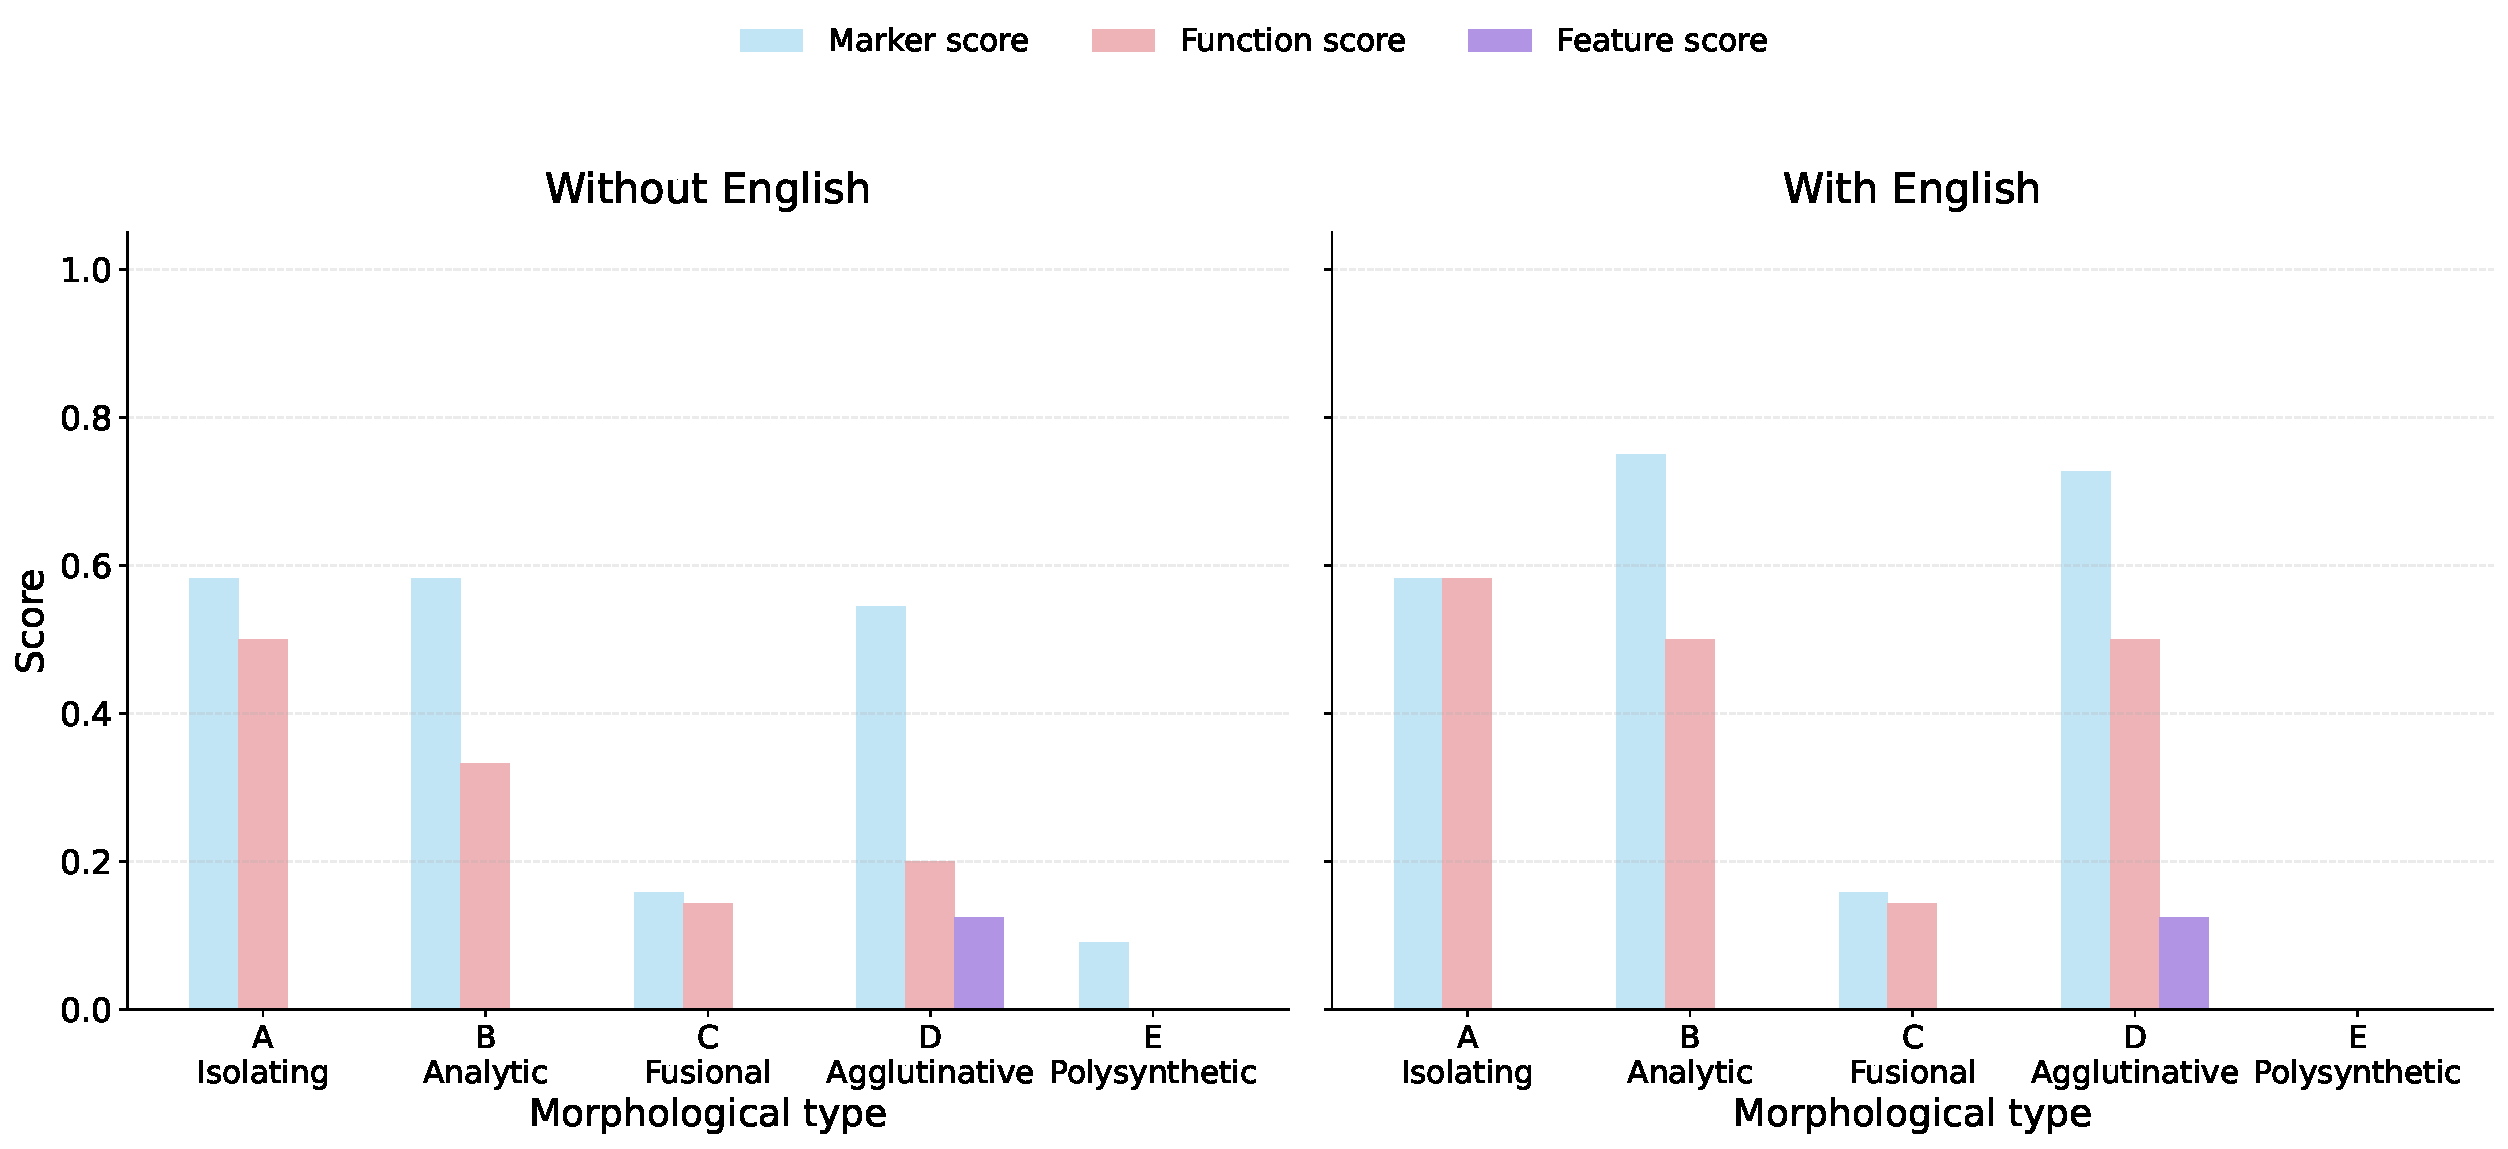
\includegraphics[width=\textwidth]{figures/figure_1_performance_by_language_type.pdf}
    \caption{Performance by morphological type. The figure reports one marker score, one function score, and one feature score for each language, with separate panels for the two experimental conditions.}
    \label{fig:performance-by-type}
\end{figure*}

\begin{table*}[t]
    \centering
    \small
    \caption{Mean scores by experimental condition.}
    \label{tab:condition-means}
    \begin{tabular}{lrrr}
        \toprule
        Metric & Without English & With English & Difference \\
        \midrule
        Type & 0.200 & 0.200 & 0.000 \\
        Marker & 0.392 & 0.444 & +0.052 \\
        Function & 0.235 & 0.345 & +0.110 \\
        Feature & 0.025 & 0.025 & 0.000 \\
        Overall & 0.213 & 0.253 & +0.040 \\
        \bottomrule
    \end{tabular}
\end{table*}

\begin{table*}[t]
    \centering
    \small
    \caption{Language-level overall scores and typological classification accuracy.}
    \label{tab:language-results}
    \begin{tabular}{llrrr}
        \toprule
        Language & Intended type & Without English & With English & Type correct \\
        \midrule
        A & Isolating & 0.271 & 0.292 & 0/2 \\
        B & Analytic & 0.229 & 0.312 & 0/2 \\
        C & Fusional & 0.075 & 0.075 & 0/2 \\
        D & Agglutinative & 0.468 & 0.588 & 2/2 \\
        E & Polysynthetic & 0.023 & 0.000 & 0/2 \\
        \bottomrule
    \end{tabular}
\end{table*}

\noindent

\begin{table*}[t]
    \centering
    \footnotesize
    \setlength{\tabcolsep}{3pt}
    \renewcommand{\arraystretch}{1.15}
    \caption{Qualitative analysis of feature interpretation by artificial language. The feature score only evaluates agreement with the predefined structured fields; this table also records relevant observations that were not necessarily counted numerically.}
    \label{tab:qualitative-features}
    \begin{tabularx}{\textwidth}{@{}>{\raggedright\arraybackslash}p{0.7cm} >{\raggedright\arraybackslash}p{1.6cm} X X@{}}
        \toprule
        Lang. & Intended type & Patterns identified & Main difficulty \\
        \midrule
        A & Isolating & Recurring temporal and spatial forms, including \texttt{vek}, \texttt{tun}, \texttt{du}, \texttt{ri}, and \texttt{na}. & Separate particles were often treated as affixes, and the absence of affixation was not recognized consistently. \\
        B & Analytic & Recurring tense and location forms, including \texttt{zo}, \texttt{ki}, \texttt{mu}, and \texttt{nel}; English made some form--meaning contrasts more visible. & Free auxiliary-like and adpositional elements were confused with suffixes, and some functions were misassigned. \\
        C & Fusional & Systematic contrasts such as \texttt{medaka}, \texttt{ardaka}, \texttt{ukdaka}, \texttt{tidaka}, and \texttt{eldaka}, showing variation with person and tense. & Person--tense fusion in prefixes was interpreted as agglutinative suffixation. \\
        D & Agglutinative & Transparent suffixes such as \texttt{-ka}, \texttt{-ra}, \texttt{-si}, \texttt{-mu}, and \texttt{-ne}, including chains such as \texttt{daka-ka-ra}. & This was the strongest analysis, although the numerical score did not capture every correct observation. \\
        E & Polysynthetic & Long recurring forms and contrasts such as \texttt{madaka}, \texttt{madakarufila}, and \texttt{madakasesena}. & Subject prefixation, object and location incorporation, and the broader polysynthetic organization were not reliably identified. \\
        \bottomrule
    \end{tabularx}
\end{table*}

The model succeeded in segmenting the correct morphemes. It also succeeded at finding some grammatical functions. Its weakest performance concerned the overall understanding of the languages' broader grammatical organization. The qualitative results for this aspect show that the model made many mistakes, but still identified some correct patterns \textbf{(Table~\ref{tab:qualitative-features})}.

All languages were classified as the ``agglutinative'' morphological type by the model.

The isolating language achieved good results for the segmentation and the best results for the grammatical functions \textbf{(Figure~\ref{fig:performance-by-type})}. The main issue is that its grammatical type was not understood by the model. The model saw affixation where there were none, interpreting the language as agglutinative \textbf{(Table~\ref{tab:qualitative-features})}. Overall, it was the third best language.

The analytic language achieved good results for the segmentation and the grammatical functions \textbf{(Figure~\ref{fig:performance-by-type})}. The main issue is that its grammatical type was not understood by the model. The model saw suffixes where there were free auxiliary-like and adpositional elements \textbf{(Table~\ref{tab:qualitative-features})}, interpreting the language as agglutinative. Overall, it was the second best language.~

The fusional language achieved relatively poor results for the segmentation and the grammatical function \textbf{(Figure~\ref{fig:performance-by-type})}. The main issue is that its grammatical type was not understood by the model. The model saw agglutinative suffixation, interpreting the language as agglutinative \textbf{(Table~\ref{tab:qualitative-features})}. Overall, the language did not perform well, ranking fourth out of five.~

The agglutinative language achieved good results for the segmentation and relatively good results on the grammatical functions \textbf{(Figure~\ref{fig:performance-by-type})}. The model performed especially well in the broader understanding of this language. It even identified additional correct patterns that were credited in the score, exceeding our expectations \textbf{(Table~\ref{tab:qualitative-features})}. It was taken as the default type choice for all languages, and it was therefore the only language whose morphological type was correctly identified.

The polysynthetic language achieved poor results for the segmentation and very poor results for the grammatical functions \textbf{(Figure~\ref{fig:performance-by-type})}. The model did not understand its broader construction at all. Overall, it was the weakest-performing language.~

The English translation improved the segmentation task for analytic and agglutinative languages, did not change the results for isolating and fusional languages, and sharply decreased performance for the polysynthetic language \textbf{(Figure~\ref{fig:performance-by-type})}. Overall, English translation improved the marker score from 0.392 to 0.444, an increase of 0.052 \textbf{(Table~\ref{tab:condition-means})}.

The English translation improved the function task for analytic, isolating and agglutinative languages. It did not change the results for the fusional or the polysynthetic language (the latter already performing poorly). \textbf{(Figure~\ref{fig:performance-by-type})} Overall, across all languages, English translation produced the largest improvement on this task~ (+0.110) \textbf{(Table~\ref{tab:condition-means})}.

The type and feature tasks were not affected by the English translation.~

The English translations improved the overall results of the isolating, analytic and agglutinative languages, did not change the results for the fusional language, and reduced the overall score for the polysynthetic language to 0.~

\section{Discussion}

The most striking finding of this study is the strong performance advantage of the agglutinative language over the other morphological types. This preference was pronounced enough to become a classification bias: despite being prompted with each language separately and instructed not to compare columns, the model classified every language as agglutinative. One possible explanation is that the recurring and relatively separable suffixes of the agglutinative language provided a particularly salient morphological pattern for the model. The results support our hypothesis that the isolating, analytic, and agglutinative languages would perform better on several measures than the fusional and polysynthetic languages, a pattern that is compatible with the literature on morphological transparency \citep{dressler2005}. English translations improved the results for the isolating, analytic, and agglutinative languages. Because they helped mainly when the model was already performing relatively well without them, they appear to have refined partially successful analyses rather than resolved the difficulties posed by the most morphologically complex languages. This finding also supports the logic of our method: the results suggest that morphological structure remained central to the model's performance, while English translations primarily provided semantic grounding when the morphological structure was already sufficiently recoverable.

\section{Limits}

There are several limitations to this article. First, although the artificial languages were designed to represent distinct morphological types, they remain relatively regular and systematic. Real languages typically exhibit greater irregularity, which is not fully captured in the present design.

Because we deliberately used small samples to test Chomsky's hypothesis that LLMs, unlike children, require very large amounts of data, some forms did not recur frequently enough for the model to identify them reliably.~

A strong classification bias toward the agglutinative category emerged, which is an important finding. However, the experiment would need to be replicated with multiple independently generated sets of artificial languages to determine whether this reflects a systematic model bias rather than a result specific to the particular languages used here.~

Finally, we tested only one model, and the study would benefit from replication with additional models to assess whether the results generalize. It would also benefit from having the scoring performed by multiple independent raters to establish inter-rater reliability.~

\section{Conclusion}

Overall, the model achieved moderate performance in marker identification and grammatical-function assignment, with the strongest results observed for three of the five languages. It recovered several local regularities for some languages, but generally struggled to reconstruct their broader grammatical organization. The clearest exception was the agglutinative language, for which the model identified both recurring local patterns and several aspects of the broader system.

Our results provide a limited perspective on Steven T. Piantadosi's ``maybe'': ``maybe theories of grammar should respect human unparalleled memory capacity for sequential material.'' Although the model had extensive prior knowledge of natural languages, it had no prior exposure to the artificial languages used here. Its success in recovering some recurring patterns from sequences alone is compatible with the possibility that sequential generalization can support at least a limited form of grammatical induction. This support is nevertheless conditional: the model performed poorly on the fusional and polysynthetic languages and did not recover enough of the broader grammatical organization of the analytic and isolating languages. The results obtained for the agglutinative language are promising for Piantadosi's proposal that grammatical knowledge may partly emerge from the generalization of sequential patterns.

These results do not settle the broader debate about human grammatical learning because they do not exclude the possibility that mechanisms beyond sequential generalization contribute to human acquisition. The findings instead suggest that sequential information can support partial grammatical inference, while access to the broader structural properties of the language continues to shape the success of that inference.

Code and data are available in an anonymized repository at \url{https://anonymous.4open.science/r/llm-artificial-languages-morphology-61FB/README.md}.

\begin{thebibliography}{}

\bibitem[Chomsky(1965)]{chomsky1965}
Chomsky, N. (1965). \emph{Aspects of the Theory of Syntax}. MIT Press.

\bibitem[Chomsky et al.(2023)]{chomskyrobertswatumull2023}
Chomsky, N., Roberts, I., \& Watumull, J. (2023). The false promise of ChatGPT. \emph{The New York Times}.

\bibitem[Dressler(2005)]{dressler2005}
Dressler, W. U. (2005). Morphological typology and first language acquisition: Some mutual challenges. In G. Booij, E. Guevara, A. Ralli, S. Sgroi, \& S. Scalise (Eds.), \emph{Morphology and Linguistic Typology: On-line Proceedings of the Fourth Mediterranean Morphology Meeting (MMM4)}. University of Bologna.

\bibitem[Louwerse(2018)]{louwerse2018}
Louwerse, M. M. (2018). Knowing the meaning of a word by the linguistic and perceptual company it keeps. \emph{Topics in Cognitive Science, 10}(3), 573--589. https://doi.org/10.1111/tops.12349

\bibitem[Millière and Buckner(2026)]{millierebuckner2026}
Millière, R., \& Buckner, C. (2026). The philosophy of language models. \emph{Philosophy Compass}. https://doi.org/10.1111/phc3.70095

\bibitem[Piantadosi(2024)]{piantadosi2024}
Piantadosi, S. T. (2024). Modern language models refute Chomsky's approach to language. In E. Gibson \& M. Poliak (Eds.), \emph{From fieldwork to linguistic theory: A tribute to Dan Everett} (pp.~353--414). Language Science Press.

\bibitem[Sveinsson(2023)]{sveinsson2023}
Sveinsson, O. (2023). \emph{Chomsky vs.~ChatGPT: An examination of Chomsky's Universal Grammar in the age of large language models}. University of Iceland.

\end{thebibliography}

\end{document}
